\documentclass[conference,a4paper]{IEEEtran}
% IEEEtran provides the IEEE layout: two columns, 10 pt Times, section headings
% ("I. INTRODUCTION", "A. Subsection"), "Fig." and "TABLE I" captions, and
% references to subsections printed as "Section III-A".

% ----------------------------------------------------------------- Fonts
\usepackage[T1]{fontenc}
\usepackage[utf8]{inputenc}
% Times text and math. newtx is preferred; mathptmx is a fallback that ships
% with every TeX distribution.
\IfFileExists{newtxtext.sty}
  {\usepackage{newtxtext}\usepackage{newtxmath}}
  {\usepackage{mathptmx}\usepackage{amssymb}}
\usepackage{microtype}
\setlength{\emergencystretch}{2em}

% ---------------------------------------------------------------- Content tools
\usepackage{amsmath}
\interdisplaylinepenalty=2500   % recommended by IEEEtran when using amsmath
\usepackage{graphicx}
\usepackage{booktabs}
\usepackage{array}
\usepackage{enumitem}
\usepackage{listings}
\usepackage{xcolor}
\usepackage{balance}   % equal-height columns on the last page (IEEE style)

% Figures generated by assignment_4/plot_results.py. They are 5.6 in wide and
% designed for a 3.5 in column, so \includegraphics[width=\columnwidth] prints
% them at the intended size (see common/plotting_style.md).
\graphicspath{{../results/}}
\newcommand{\figwidth}{\columnwidth}

\lstset{basicstyle=\footnotesize\ttfamily, frame=lines, framesep=3pt,
        columns=fullflexible, keepspaces=true, xleftmargin=0pt, xrightmargin=0pt}

% Links in the deep blue of the C OpenMP series in the figures.
\definecolor{linkblue}{HTML}{1F43B2}
\usepackage[colorlinks=true,linkcolor=linkblue,citecolor=linkblue,urlcolor=linkblue]{hyperref}
\hypersetup{pdftitle={Distributed Matrix Multiplication},
            pdfauthor={Javier Ruano Hernández}}

% ------------------------------------------------------------------ Shortcuts
\newcommand{\bigO}[1]{\mathcal{O}\!\left(#1\right)}
\newcommand{\code}[1]{\texttt{#1}}
\newcommand{\dist}{\code{distributed}}
\newcommand{\seqpy}{\code{seq\_python}}
\newcommand{\cseq}{\code{c\_baseline}}
\newcommand{\comp}{\code{c\_omp\_tiled}}
\newcommand{\Tdist}{T_{\mathrm{dist}}}
\newcommand{\Tnp}{T_{\mathrm{NumPy}}}

% =============================================================================
\title{Distributed Matrix Multiplication:\\Scaling and Overhead on a Local Dask Cluster}
\author{\IEEEauthorblockN{{Javier Ruano Hernández}}
\IEEEauthorblockA{Big Data -- Assignment 4\\
Universidad de Las Palmas de Gran Canaria (ULPGC)\\
Code and data: \url{https://github.com/javierruanohdez/big-data-assignments/tree/main/assignment_4}}}

\begin{document}
\maketitle

% =============================================================================
% ABSTRACT
% =============================================================================
% All numbers in this report are computed from results/measurements.csv
% (115 runs) and match results/results_summary.md. Recompute them if you
% re-run the benchmark.
\begin{abstract}
We implement a 2D block-partitioned dense matrix multiplication on a local
Dask cluster of $p$ single-threaded worker processes and measure how it scales
and where its time goes. Tiles follow a 2D block-cyclic distribution; each
output tile is computed by its owner, and input tiles travel between workers
along process rows and columns. On a laptop with 4 cores and 8 hardware threads
under WSL~2, we ran strong scaling ($n = 2000$, 4000; $p = 1$--8), weak scaling
($n_p = 1000\,p^{1/3}$) and a comparison with the sequential and OpenMP C
programs of earlier assignments. At $n = 4000$, the end-to-end time fell from
7.65~s on one worker to 3.69~s on four ($S = 2.08$, $E = 52\%$) and rose to
4.07~s on eight. The same tile algorithm in one NumPy process took 4.05~s:
distribution paid off only there, by a factor of 1.10. Dask added 4.6--6.5~ms
per task, scatter and gather through the single client took 10--25\% of the
time, and cluster start-up 9--16~s. Under weak scaling, efficiency fell to 52\%
at $p = 8$ while the traffic between workers grew from 0 to 128~MB, exactly as a
$4pn^2$-byte model predicts. At $n = 2000$, Dask (0.697~s) beat C OpenMP
(1.07~s) and the C baseline (13.7~s), but one NumPy process was faster still
(0.648~s): the BLAS kernel, not the distributed paradigm, explains the gain.
These results describe one machine.
\end{abstract}

\begin{IEEEkeywords}
distributed computing, matrix multiplication, Dask, task scheduling, block
partitioning, strong scaling, weak scaling, communication overhead.
\end{IEEEkeywords}

% =============================================================================
\section{Introduction and Objective}
\label{sec:intro}
% =============================================================================

Assignments~2 and~3 made dense matrix multiplication cache-friendly and then
parallel: on the test machine, OpenMP threads ran the tiled kernel at
$n = 2000$ in 1.06~s with eight threads, and in 0.445~s with explicit SIMD.
Those threads share one address space. Distributed frameworks such as MPI,
Spark or Dask scale beyond one machine by giving each worker process its own
memory, so a worker that needs another's data must receive it as a serialised
message. This assignment ports the block multiplication to the Dask
distributed scheduler~\cite{rocklin2015} and measures what that model costs.

\paragraph{Objective} We answer the following research question:
\begin{quote}
\emph{How does a 2D block-partitioned matrix multiplication on a multi-process
task framework scale with the number of worker processes, and how much of its
time goes to computation, and how much to partitioning, serialisation, data
transfer and scheduling?}
\end{quote}
\begin{enumerate}[label=\textbf{RQ\arabic*.}, leftmargin=3.2em, itemsep=1pt]
  \item How do speedup and efficiency evolve with $p$ for a fixed problem?
  \item How is the time divided between setup, scatter, computation and gather?
  \item How do time and communication grow when the work per worker is
        constant (weak scaling)?
  \item How does the distributed program compare with the sequential and
        OpenMP C programs, and with the same algorithm in one process?
\end{enumerate}

\paragraph{Hypotheses} \textbf{H1}: on one machine, the framework's costs
(scheduling, serialisation, transfers) make Dask slower than the identical tile
algorithm in one process, except where large problems amortise them.
\textbf{H2}: strong scaling saturates at the four physical cores, since further
workers share cores (SMT) with each other and with the driver process.
\textbf{H3}: under weak scaling the time grows with $p$, because the data each
worker receives grows and all input and output pass through one client.

\paragraph{Contributions} (i)~A distributed implementation with explicit
partitioning, placement, communication and collection; (ii)~a single-process
baseline with the same tiles and kernel; (iii)~a timing design that separates
one-time, end-to-end and per-phase costs; and (iv)~a communication model that
matches the measured traffic exactly.

% =============================================================================
\section{Background and References}
\label{sec:background}
% =============================================================================

\subsection{2D Block Partitioning}
Cutting the $n \times n$ matrices into $b \times b$ tiles, $n_b = \lceil n/b
\rceil$ per side, turns $C = AB$ into the same formula on sub-matrices:
\begin{equation}
  C_{IJ} = \sum_{K=0}^{n_b-1} A_{IK}\, B_{KJ}.
  \label{eq:blocks}
\end{equation}
With one task per triple $(I, J, K)$ there are $n_b^3$ tasks; the $n_b$ tasks
of one output tile form a chain (each adds to the previous partial sum), and
the $n_b^2$ chains are independent. A task performs $2b^3$ floating-point
operations on two tiles of $8b^2$ bytes, 62.5 operations per byte for
$b = 500$: compute-bound in the roofline model~\cite{williams2009}, a regime
where optimised BLAS approaches peak~\cite{goto2008}.

\subsection{Distribution and Communication Complexity}
\label{sec:bg-comm}
Distributed algorithms arrange $p$ processes in a $p_r \times p_c$ grid. In the
2D block-cyclic layout of ScaLAPACK~\cite{blackford1997}, tile $(I, J)$ belongs
to process $(I \bmod p_r,\, J \bmod p_c)$. Cannon's algorithm~\cite{cannon1969}
and SUMMA~\cite{vandegeijn1997} let each process compute its own tiles of $C$
while tiles of $A$ travel along process rows and tiles of $B$ along columns; on a
$\sqrt{p} \times \sqrt{p}$ grid each process receives $\bigO{n^2/\sqrt{p}}$
words, which matches the lower bound for algorithms that store each matrix
once~\cite{irony2004}. In our owner-computes scheme
(Section~\ref{sec:impl}), a worker needs the $A$ tiles of its tile rows and the
$B$ tiles of its tile columns, except those it already holds:
\begin{equation}
  W = n^2 \left[\frac{1}{p_r}\Big(1 - \frac{1}{p_c}\Big)
             + \frac{1}{p_c}\Big(1 - \frac{1}{p_r}\Big)\right]
  \label{eq:comm}
\end{equation}
elements per worker. For the grids $1 \times 2$, $2 \times 2$ and $2 \times 4$
used here, $W = n^2/2$, so the workers receive $8pW = 4pn^2$ bytes in total.
The client additionally sends $A$ and $B$ ($16n^2$ bytes) and receives $C$
($8n^2$ bytes). Per worker, communication ($4n^2$ bytes) thus grows relative to
computation ($2n^3/p$ operations) as $p/n$.

\subsection{Task-Graph Scheduling}
Dask represents a computation as a graph of tasks~\cite{rocklin2015,dask2016}.
In its distributed scheduler, a central scheduler process tracks every task and
datum, assigns ready tasks to workers and tells them where their inputs live;
workers run tasks and fetch missing inputs directly from each other. The client
submits tasks and holds \emph{futures}, handles to results that stay on the
workers. Coordinating one task costs the scheduler about a
millisecond~\cite{daskeff}. NumPy arrays cross process boundaries as raw buffers
with a small header, but each transfer still copies the bytes through both
processes and the network stack. Python's global interpreter lock (GIL) lets
one thread per process run Python code at a time; separate processes avoid
sharing it, and NumPy releases it inside BLAS, but a worker's communication and
task threads still take turns for it.

\subsection{Speedup, Amdahl's Law and Weak Scaling}
With $T_p$ the time on $p$ workers, the self-relative speedup and efficiency are
\begin{equation}
  S(p) = \frac{T_1}{T_p}, \qquad E(p) = \frac{S(p)}{p}.
  \label{eq:speedup}
\end{equation}
If a fraction $f$ of the work is serial, Amdahl's law bounds
$S(p) \le 1/(f + (1-f)/p)$~\cite{amdahl1967}; the Karp--Flatt
metric~\cite{karp1990}
\begin{equation}
  e = \frac{1/S(p) - 1/p}{1 - 1/p}
  \label{eq:karpflatt}
\end{equation}
is the serial fraction that would explain a measured speedup; it absorbs every
loss (overheads, contention, imbalance). Following
Gustafson~\cite{gustafson1988}, weak scaling grows the problem with $p$ so that
the work per worker is constant; with $2n^3$ operations, this means
\begin{equation}
  n_p = n_1\, p^{1/3}, \qquad E_w(p) = \frac{T(1, n_1)}{T(p, n_p)},
  \label{eq:weak}
\end{equation}
with ideal $E_w = 1$ (constant time). By \eqref{eq:comm}, the data received per
worker then grows as $4n_p^2 = 4n_1^2\, p^{2/3}$ bytes, and the total as
$p^{5/3}$.

% =============================================================================
\section{Methodology}
\label{sec:method}
% =============================================================================

\subsection{Experimental Environment}
\label{sec:environment}
All measurements were taken on the machine of Table~\ref{tab:environment}, the
one used in Assignments~1--3, connected to mains power with other applications
closed. Its four cores are of two types, one Zen~5 and three Zen~5c cores with
lower maximum clocks~\cite{nbc330}.

\begin{table}[t]
  \centering
  \caption{Hardware and software environment}
  \label{tab:environment}
  \footnotesize
  % Sources: lscpu and the CPU specification (as in Assignment 3, same machine);
  % uname -r, gcc --version, python3 --version and the package versions of the
  % project's virtual environment, checked when the benchmark was run.
  \begin{tabular}{@{}l>{\raggedright\arraybackslash}p{0.64\columnwidth}@{}}
    \toprule
    \textbf{Item} & \textbf{Value} \\
    \midrule
    CPU model               & AMD Ryzen AI 5 330 w/ Radeon 820M \\
    Cores / logical threads & 4 cores (1 Zen~5 + 3 Zen~5c) / 8 threads (2-way SMT) \\
    Clock                   & 2.0~GHz base; boost up to 4.5~GHz (Zen~5 core)
                              and 3.4~GHz (Zen~5c cores) \\
    Caches                  & L1d 48~KiB, L2 1~MiB per core; L3 8~MiB shared \\
    RAM                     & 15~GiB (available to WSL~2) \\
    Operating system        & Ubuntu 26.04 LTS on WSL~2 \\
    Kernel                  & 6.18.33.2-microsoft-standard-WSL2 \\
    C compiler / OpenMP     & GCC 15.2.0 with libgomp \\
    Python                  & CPython 3.14.4 \\
    Python packages         & dask/distributed 2026.8.0, NumPy 2.5.5, psutil 7.2.2 \\
    \bottomrule
  \end{tabular}
\end{table}

\subsection{Execution Model: Workers, Processes and Machines}
\label{sec:model}
The program is a real distributed program on a single machine, and we keep
three levels apart. A \emph{worker} is a Dask worker
process with exactly one thread, so it executes one task at a time; NumPy's
BLAS is limited to one thread in every process. An \emph{OS process} is any
process of a run: the driver (Dask client and, in a \code{LocalCluster}, the
scheduler), $p$ workers, and one small supervisor (``nanny'') per worker,
$2p + 1$ in total. The \emph{physical machine} is one laptop: all processes run
inside one WSL~2 virtual machine and communicate over TCP on the loopback
interface. Dask's work stealing and active memory manager are disabled, so
the placement is the program's own. No worker ever reads another's memory;
every tile a worker lacks is serialised, sent through a socket and
deserialised, as between machines.

\paragraph{Local execution limitation} One machine reproduces the programming
model of a cluster, not its performance profile. Loopback has no wire: a
transfer costs serialisation and memory copies but no link bandwidth or switch
latency, so communication is optimistic. All $2p + 1$ processes share 4 cores
(8 hardware threads) and one pool of RAM, so adding workers adds neither cores
beyond four nor memory. Workers are not pinned (unlike the OpenMP threads of
Assignment~3), and Windows schedules the virtual CPUs of WSL~2.

\subsection{Implementation}
\label{sec:impl}
\paragraph{Partitioning} The client loads $A$ and $B$ from the shared binary
input files of the previous assignments and cuts them into contiguous tile
copies (edge tiles are smaller when $b$ does not divide $n$), so each tile is
serialised and sent as a single buffer.

\paragraph{Placement} The $p$ workers form the most square grid with
$p_r \le p_c$: $1 \times 1$, $1 \times 2$, $2 \times 2$ and $2 \times 4$ for
$p = 1, 2, 4, 8$. Tile $(I, J)$ of every matrix belongs to worker
$(I \bmod p_r)\, p_c + (J \bmod p_c)$. The client scatters each $A$ and $B$ tile
once to its owner (one message per worker, sent directly, not through the
scheduler), and every step of the chain for $C_{IJ}$ is pinned to the owner of
$C_{IJ}$ (Listing~\ref{lst:submit}), so partial sums never move. When $n_b$ is a
multiple of $p_r$ and $p_c$, as in all benchmark runs, every worker owns the
same number of $C$ tiles.

\begin{lstlisting}[language=Python, float=t, caption={Task submission (simplified): each step receives the previous partial sum and two input tiles; Dask fetches tiles held elsewhere.}, label=lst:submit, captionpos=b]
for I in range(nb):
 for J in range(nb):
  w = addr[owner(I, J, grid)]   # owner computes
  part = None
  for K in range(nb):           # increasing K
   part = client.submit(mult_acc, part,
            A[I, K], B[K, J], kernel, workers=[w],
            allow_other_workers=False)
  C[I, J] = part                # final tile
\end{lstlisting}

\paragraph{Communication} A task that needs a tile held elsewhere makes Dask
fetch it directly from the holder; the copy stays while tasks there still need
it, so each (tile, worker) pair crosses once, $A$ tiles along process rows and
$B$ tiles along columns, as in SUMMA. Spilling to disk and compression are
disabled, so disk I/O never enters the timings and the bytes sent equal the
array bytes.

\paragraph{Collection and kernels} Result tiles are assembled on the client
into a NaN-filled $C$, so a missing tile cannot go unnoticed. The benchmark
kernel is NumPy's \code{matmul} (BLAS \code{dgemm}, one thread), what a
production system runs on each node. A verification-only kernel adds rank-1
updates in increasing $k$, which reproduces the summation order of the C
programs; it is about 20 times slower.

\subsection{Compared Implementations and Their Differences}
\label{sec:baselines}
The four modes run on the same input files: \dist{} ($p$ worker processes)
and \seqpy{} (one process) multiply NumPy tiles; \cseq{} is the scalar i-j-k
loop of Assignments~1--2 (C, \code{-O2}, one thread); \comp{} is the tiled
OpenMP kernel of Assignment~3 (C, \code{-O3 -march=native}, $b = 64$, $p$
pinned threads). They differ in more than the parallel model:
\begin{itemize}[itemsep=1pt]
  \item \textbf{Kernel.} Dask and NumPy run optimised BLAS (vector
        instructions, fused multiply-add, register blocking~\cite{goto2008});
        both C programs keep scalar inner loops.
  \item \textbf{Runtime.} Python only orchestrates; the arithmetic runs in
        compiled BLAS. Dask adds serialisation, sockets and a scheduler; OpenMP
        threads share memory and synchronise in microseconds.
  \item \textbf{Timed region.} The C programs time their kernel only; the Dask
        time also contains partitioning, scatter and gather, which a
        distributed computation cannot avoid.
\end{itemize}
\seqpy{} isolates the effect of distribution: same tiles, same kernel calls,
same order, no Dask.

\subsection{Experimental Design}
\label{sec:design}
Table~\ref{tab:parameters} lists the parameters. The strong-scaling tile
edge is fixed across $p$, so the same tasks are only distributed differently;
one task takes 7--9~ms with single-threaded BLAS, well above the documented
scheduling cost. The weak-scaling tile grid is fixed at $4 \times 4$ (16 $C$
tiles, 64 tasks), so the tile edge grows with $n_p$.

\begin{table}[t]
  \centering
  \caption{Fixed experimental parameters}
  \label{tab:parameters}
  \footnotesize
  \begin{tabular}{@{}l>{\raggedright\arraybackslash}p{0.70\columnwidth}@{}}
    \toprule
    \textbf{Parameter} & \textbf{Value} \\
    \midrule
    Strong scaling & $n$ = 2000 ($4 \times 4$ tiles, 64 tasks) and 4000
                     ($8 \times 8$ tiles, 512 tasks); $b = 500$; $p$ = 1, 2, 4, 8 \\
    Weak scaling   & $n_p = \mathrm{round}(1000\, p^{1/3})$ = 1000, 1260, 1587, 2000;
                     $b_p = \lceil n_p/4 \rceil$ = 250, 315, 397, 500 \\
    References     & \seqpy{} at every $n$; \cseq{} and \comp{}
                     ($p$ = 1, 2, 4, 8) at $n = 2000$ \\
    Cluster        & \code{LocalCluster(n\_workers=p, threads\_per\_worker=1,
                     processes=True)}, 1 BLAS thread per process \\
    Repetitions    & 5 per configuration, each a fresh process; 300~s budget \\
    Inputs         & uniform in $[-1, 1)$, base seed 42, shared binary files \\
    Timer / memory & \code{time.perf\_counter}; peak RSS per process
                     (\code{VmHWM}; GNU \code{time} for C) \\
    \bottomrule
  \end{tabular}
\end{table}

\subsection{Timing Boundaries}
\label{sec:timing}
Each repetition is a fresh process that starts a new cluster and measures, in
order: (i)~\emph{setup}: cluster and client start, plus one run of the whole
task graph on $1 \times 1$ tiles, which opens every connection and ships the
task function (like thread creation in the C programs, it lies outside the main
timer); (ii)~a \emph{cold} pipelined pass on the fresh processes, reported but
not used as the main metric; (iii)~the \emph{end-to-end} time $T$: a pipelined
pass on warm workers without any barrier, from partitioning to the assembled
$C$, collecting each result tile as soon as it is ready; and (iv)~a
\emph{barriered} pass that waits after each phase: \emph{scatter} (partition and
send the tiles), \emph{compute} (all tasks, including worker-to-worker
transfers) and \emph{gather} (fetch and assemble $C$). Loading the input file
is outside every timer.

The barriered phases are not additive parts of $T$. In the pipelined pass,
activities overlap: tasks start while others are still being submitted, and
finished tiles travel to the client while others are computed. But tiles are
also collected one at a time instead of in one batch, and the driver then
competes with the workers for CPU; the barriers add their own round trips.
The phase sum can thus be larger or smaller than $T$: the barriered pass shows
\emph{where} the time goes, only the pipelined pass \emph{how long} a
multiplication takes.

\subsection{Metrics}
\label{sec:metrics}
$S(p)$ and $E(p)$ follow \eqref{eq:speedup} with median end-to-end times. Since
$T_1$ already contains Dask's overhead, we also report the gain over the same
algorithm in one process, $G(p) = \Tnp / \Tdist(p)$ ($G > 1$: distribution paid
off), $E_w$ from \eqref{eq:weak}, and the cross-paradigm ratios
$T_{\mathrm{C,seq}}/T$ and $T_{\mathrm{C,OpenMP}}(p)/\Tdist(p)$. We report
medians and interquartile ranges (IQR $= Q_3 - Q_1$) over five
repetitions~\cite{georges2007}; ratios use medians. Inter-worker
traffic is computed from the placement plan and, independently, summed from
each worker's transfer log during the barriered pass. All statistics and figures
are produced by \code{plot\_results.py} from the raw data.

\subsection{Validation}
\label{sec:validation}
Before benchmarking, \code{verify\_correctness.py} ran every mode on six cases:
$A \times I$, $A \times 0$, a hand-computed $3 \times 3$ product, and random
inputs with $n = 10$, 100 and 131, with three tile edges per case ($\lfloor n/3
\rfloor$: uneven edge tiles and a tile grid that wraps around the $2 \times 2$
process grid; $\lceil n/2 \rceil$; and $n + 5$: one tile, idle workers),
$p = 1, 2, 4$, both kernels and both passes. Results were compared with a
correctly rounded \code{math.fsum} reference, $|x - x_{\text{ref}}| \le 100\,
n^2 u + 10^{-12} |x_{\text{ref}}|$ with $u = 2^{-53}$~\cite{higham2002}. All 279
runs passed (largest error $1.07 \times 10^{-14}$); the order-preserving kernel
was bit-identical to the C baseline in every run, proving that tiling,
placement and collection lose or duplicate nothing; and the measured
inter-worker bytes equalled the plan. An injected bug (one missing step per
chain) failed all three checks.

% =============================================================================
\section{Results}
\label{sec:results}
% =============================================================================

All 115 runs (23 configurations, 5 repetitions) completed, with no timeouts,
errors or checksum mismatches; every mode printed the same 11-digit checksum
for each input. Times are in seconds; data volumes in MB $= 10^6$ bytes; memory
in MB $= 2^{20}$ bytes.

\begin{figure}[t]
  \centering
  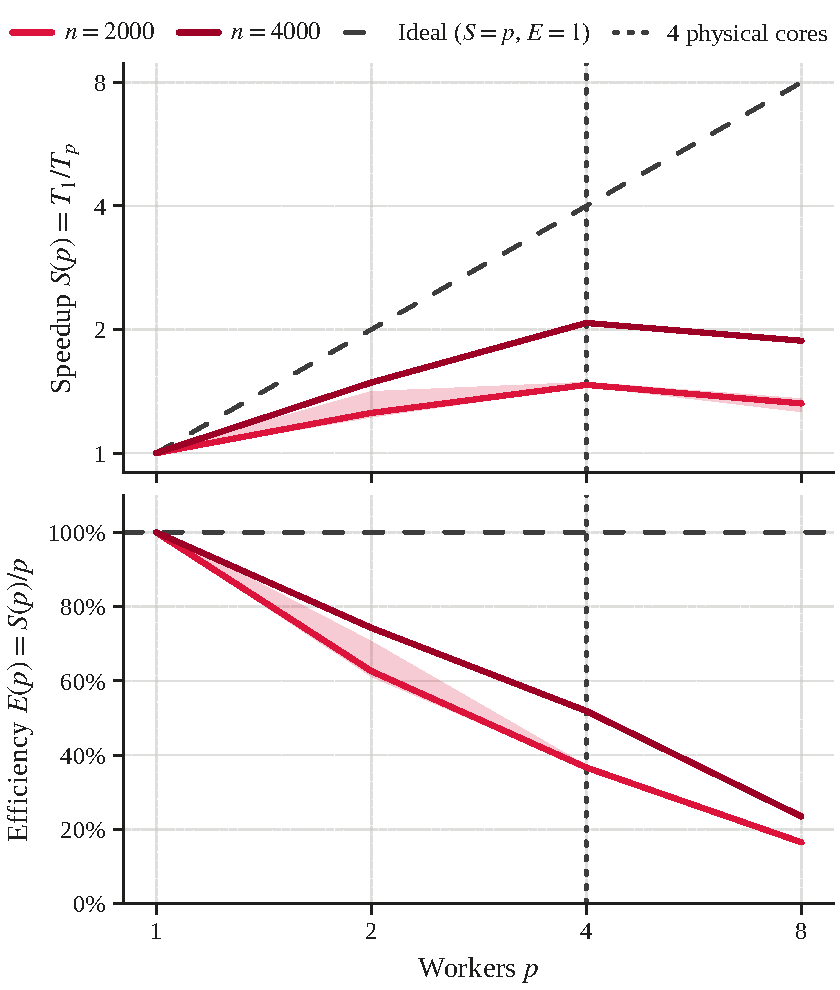
\includegraphics[width=\figwidth]{strong_scaling_speedup_efficiency.pdf}
  \caption{Strong scaling: self-relative speedup $S(p) = T_1/T_p$ (top, log-log)
           and efficiency (bottom) of the Dask program, median of five runs with
           IQR bands. Dashed: ideal. Dotted: the 4 physical cores.}
  \label{fig:strong}
\end{figure}

\begin{table}[t]
  \centering
  \caption{Strong scaling: median end-to-end time and IQR, self-relative
           speedup and efficiency, and gain over the same algorithm in one
           NumPy process}
  \label{tab:strong}
  \footnotesize
  \setlength{\tabcolsep}{4.5pt}
  \begin{tabular}{@{}rlrrrrrr@{}}
    \toprule
    $n$ & Mode & $p$ & Median & IQR & $S(p)$ & $E(p)$ & $G(p)$ \\
    \midrule
    2000 & \seqpy & 1 & 0.648 & 0.028  & --   & --    & --   \\
         & \dist  & 1 & 1.021 & 0.012  & 1.00 & 100\% & 0.63 \\
         &        & 2 & 0.815 & 0.11   & 1.25 & 63\%  & 0.80 \\
         &        & 4 & 0.697 & 0.015  & 1.47 & 37\%  & 0.93 \\
         &        & 8 & 0.773 & 0.057  & 1.32 & 17\%  & 0.84 \\
    \midrule
    4000 & \seqpy & 1 & 4.049 & 0.048  & --   & --    & --   \\
         & \dist  & 1 & 7.648 & 0.020  & 1.00 & 100\% & 0.53 \\
         &        & 2 & 5.148 & 0.0092 & 1.49 & 74\%  & 0.79 \\
         &        & 4 & 3.686 & 0.078  & 2.08 & 52\%  & 1.10 \\
         &        & 8 & 4.073 & 0.043  & 1.88 & 23\%  & 0.99 \\
    \bottomrule
  \end{tabular}
\end{table}

\subsection{Strong Scaling}
\label{sec:res-strong}

Both sizes were fastest at $p = 4$ (Table~\ref{tab:strong},
Fig.~\ref{fig:strong}): $S = 2.08$ ($E = 52\%$) at $n = 4000$ and 1.47 at
$n = 2000$; eight workers were slower than four. The gain over \seqpy{}
exceeded 1 only at $n = 4000$, $p = 4$ (1.10); with one worker, Dask took 1.58
($n = 2000$) and 1.89 times ($n = 4000$) as long as the same tile algorithm in
one process. The IQR stayed below 5\% of the median except at $n = 2000$ with
$p = 8$ (7\%) and $p = 2$ (14\%).

\begin{figure}[t]
  \centering
  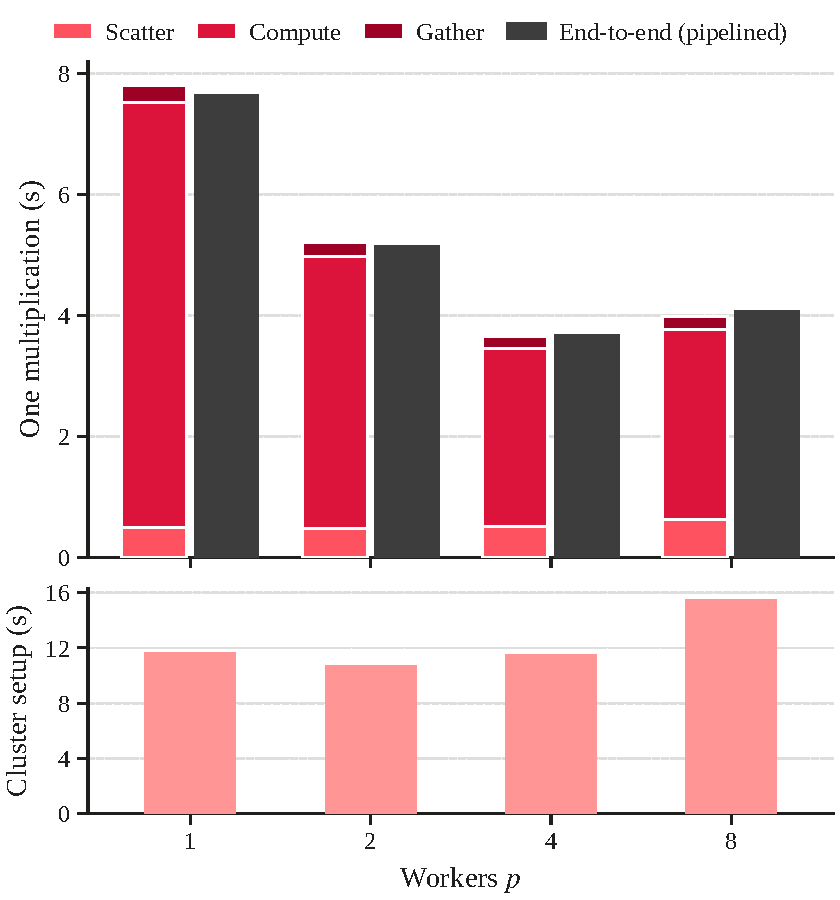
\includegraphics[width=\figwidth]{time_breakdown_n4000.pdf}
  \caption{Time per phase at $n = 4000$ (medians). Top: the barriered phases
           stacked, next to the pipelined end-to-end time. Bottom: one-time
           cluster setup, on its own scale.}
  \label{fig:breakdown}
\end{figure}

\begin{table}[t]
  \centering
  \caption{Phase breakdown (medians): setup, barriered phases, their sum, the
           pipelined end-to-end time $T$, and $\Delta = (\text{sum} - T)/T$}
  \label{tab:phases}
  \footnotesize
  \setlength{\tabcolsep}{3.1pt}
  \begin{tabular}{@{}rrrrrrrrr@{}}
    \toprule
    $n$ & $p$ & Setup & Scatter & Compute & Gather & Sum & $T$ & $\Delta$ \\
    \midrule
    2000 & 1 & 10.27 & 0.083 & 0.845 & 0.030 & 0.965 & 1.021 & $-5.5\%$ \\
         & 2 &  9.02 & 0.101 & 0.668 & 0.024 & 0.793 & 0.815 & $-2.7\%$ \\
         & 4 & 10.54 & 0.111 & 0.518 & 0.024 & 0.654 & 0.697 & $-6.1\%$ \\
         & 8 & 12.92 & 0.165 & 0.559 & 0.025 & 0.756 & 0.773 & $-2.2\%$ \\
    \midrule
    4000 & 1 & 11.70 & 0.489 & 7.032 & 0.280 & 7.697 & 7.648 & $+0.6\%$ \\
         & 2 & 10.75 & 0.484 & 4.492 & 0.229 & 5.212 & 5.148 & $+1.2\%$ \\
         & 4 & 11.50 & 0.515 & 2.931 & 0.208 & 3.671 & 3.686 & $-0.4\%$ \\
         & 8 & 15.54 & 0.624 & 3.141 & 0.213 & 3.951 & 4.073 & $-3.0\%$ \\
    \bottomrule
  \end{tabular}
\end{table}

\subsection{Where the Time Goes}
\label{sec:res-phases}

Computation dominates at $n = 4000$ (Fig.~\ref{fig:breakdown},
Table~\ref{tab:phases}) but scales poorly: the compute phase was only 2.40
times faster on four workers than on one, and slower on eight than on four. Scatter and gather, which pass every tile through the
single client, did not shrink with $p$: together they took 0.77~s (10\% of the
phase sum) at $p = 1$ and 0.84~s (21\%) at $p = 8$; at $n = 2000$ their share
grew from 12 to 25\%. Including partitioning, the client sent data at
0.39--0.77~GB/s in scatter and received it at 0.46--1.31~GB/s in gather. Setup took 9--16~s, 1.5--3.8 times one
multiplication at $n = 4000$ and 10--17 times at $n = 2000$. The cold first pass
was 3--14\% slower than the warm one at $n = 4000$ and 16--35\% at $n = 2000$.
The phase sum differed from $T$ by $-6.1$ to $+1.2\%$; in 6 of 8
configurations the pipelined pass was the slower one.

\begin{table}[t]
  \centering
  \caption{Data moved between workers per multiplication (MB; theoretical =
           measured in all 60 Dask runs) and peak memory (MB, medians)}
  \label{tab:comm}
  \footnotesize
  \setlength{\tabcolsep}{3.6pt}
  \begin{tabular}{@{}rrcrrrr@{}}
    \toprule
    & & & \multicolumn{2}{c}{\textbf{Between workers}} & \multicolumn{2}{c}{\textbf{Memory}} \\
    \cmidrule(lr){4-5} \cmidrule(l){6-7}
    $n$ & $p$ & Grid & Total & Per worker & Worker (max) & All processes \\
    \midrule
    2000 & 1 & $1 \times 1$ &   0.0 &  0.0 & 169.5 &  392 \\
         & 2 & $1 \times 2$ &  32.0 & 16.0 & 138.4 &  500 \\
         & 4 & $2 \times 2$ &  64.0 & 16.0 & 118.2 &  693 \\
         & 8 & $2 \times 4$ & 128.0 & 16.0 & 108.5 & 1072 \\
    \midrule
    4000 & 1 & $1 \times 1$ &   0.0 &  0.0 & 451.4 & 1039 \\
         & 2 & $1 \times 2$ & 128.0 & 64.0 & 331.0 & 1259 \\
         & 4 & $2 \times 2$ & 256.0 & 64.0 & 332.6 & 1878 \\
         & 8 & $2 \times 4$ & 512.0 & 64.0 & 262.9 & 2619 \\
    \bottomrule
  \end{tabular}
\end{table}

\subsection{Communication and Memory}
\label{sec:res-comm}

The traffic between workers followed \eqref{eq:comm} exactly
(Table~\ref{tab:comm}): $n^2/2$ elements per worker for $p \ge 2$, so the total
doubled with $p$ and reached 512~MB, twice the input, at $n = 4000$, $p = 8$.
The client always sent $16n^2$ bytes and received $8n^2$. One worker's peak
memory fell with $p$, but the memory of all processes grew from 1.0 to 2.6~GB at
$n = 4000$, against 0.77~GB for \seqpy{} and 93~MB for the C programs at
$n = 2000$.

\begin{figure}[t]
  \centering
  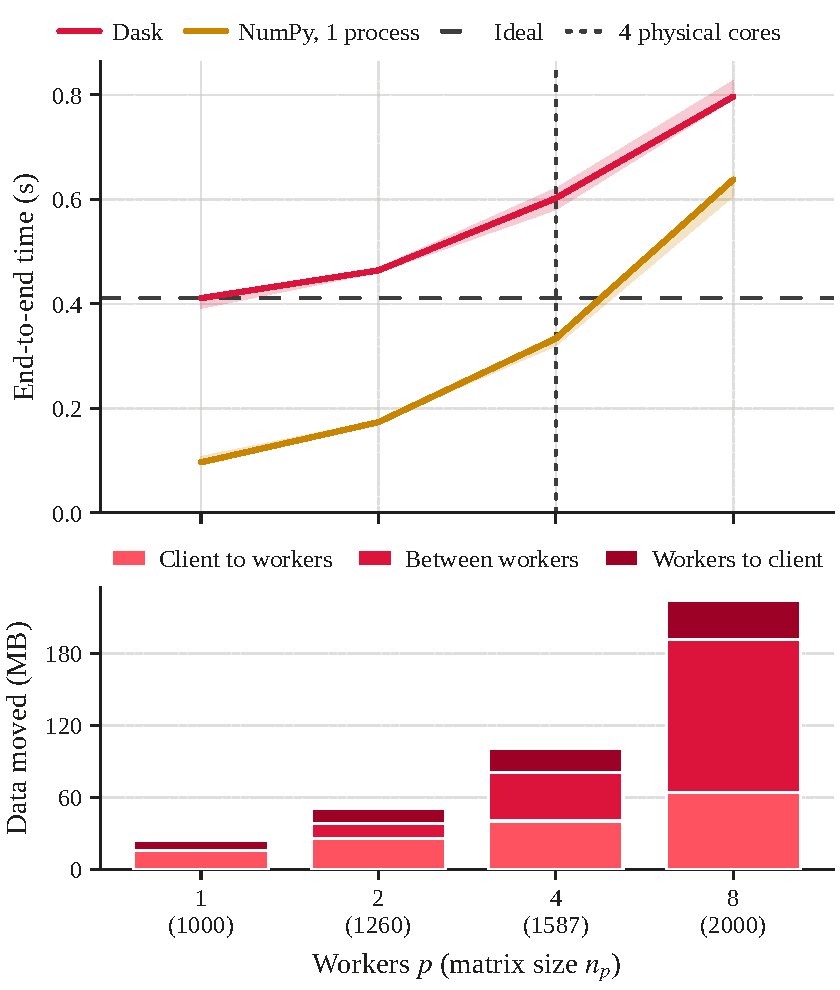
\includegraphics[width=\figwidth]{weak_scaling.pdf}
  \caption{Weak scaling ($n_p = 1000\,p^{1/3}$, same work per worker). Top:
           end-to-end time of Dask and of one NumPy process at the same $n_p$,
           medians with IQR bands; dashed: ideal constant time. Bottom: data
           moved per multiplication.}
  \label{fig:weak}
\end{figure}

\begin{table}[t]
  \centering
  \caption{Weak scaling: Dask time (median, IQR), weak efficiency, NumPy time
           at the same $n_p$, scatter time and data received per worker}
  \label{tab:weak}
  \footnotesize
  \setlength{\tabcolsep}{3.7pt}
  \begin{tabular}{@{}rrrrrrrr@{}}
    \toprule
    $p$ & $n_p$ & Median & IQR & $E_w(p)$ & NumPy & Scatter & MB/worker \\
    \midrule
    1 & 1000 & 0.411 & 0.020  & 100\% & 0.097 & 0.037 &  0.0 \\
    2 & 1260 & 0.464 & 0.0089 &  89\% & 0.174 & 0.065 &  6.4 \\
    4 & 1587 & 0.602 & 0.041  &  68\% & 0.334 & 0.105 & 10.1 \\
    8 & 2000 & 0.797 & 0.036  &  52\% & 0.638 & 0.170 & 16.0 \\
    \bottomrule
  \end{tabular}
\end{table}

\subsection{Weak Scaling}
\label{sec:res-weak}

With constant work per worker, the Dask time grew from 0.411 to 0.797~s
(Fig.~\ref{fig:weak}, Table~\ref{tab:weak}): $E_w = 52\%$ at $p = 8$. One NumPy
process doing all the work took 0.097 to 0.638~s; divided by $p$, this stayed
within 0.080--0.097~s, confirming constant work per worker. Scatter time rose
4.6-fold as the client sent 16 to 64~MB, and the data each worker received
grew from 0 to 16~MB, as the $p^{2/3}$ law predicts. Dask stayed slower than one
NumPy process at every point.

\begin{figure}[t]
  \centering
  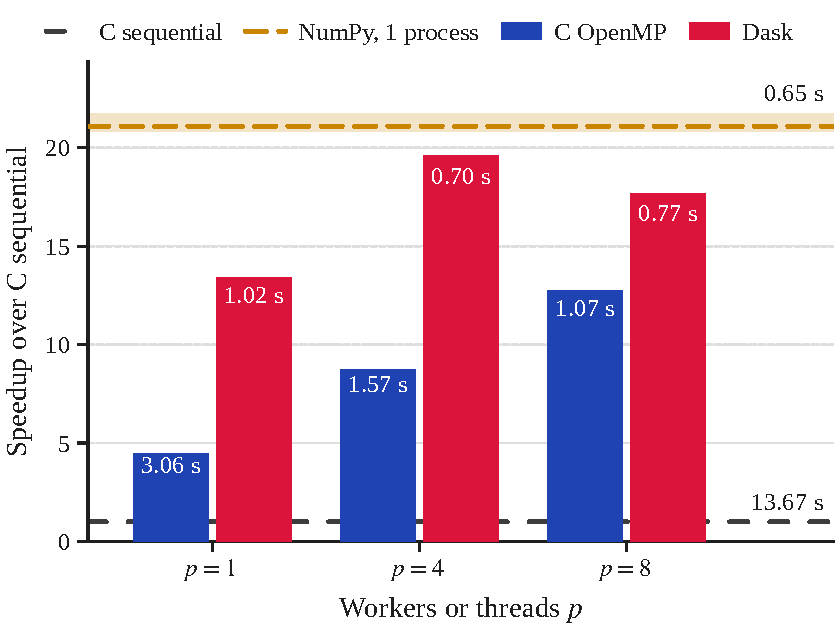
\includegraphics[width=\figwidth]{cross_paradigm_n2000.pdf}
  \caption{Speed relative to the C baseline at $n = 2000$ (median times in the
           bars). Dashed: C baseline (13.67~s) and one NumPy process (0.65~s,
           with IQR band).}
  \label{fig:cross}
\end{figure}

\begin{table}[t]
  \centering
  \caption{Cross-paradigm comparison at $n = 2000$: median time, IQR, speed
           relative to \cseq{}, and arithmetic rate ($2n^3/T$)}
  \label{tab:cross}
  \footnotesize
  \setlength{\tabcolsep}{4.5pt}
  \begin{tabular}{@{}lrrrrr@{}}
    \toprule
    Mode & $p$ & Median & IQR & vs.\ \cseq & GFLOP/s \\
    \midrule
    \cseq  & 1 & 13.67 & 0.14  &  1.00 &  1.17 \\
    \comp  & 1 & 3.060 & 0.042 &  4.47 &  5.23 \\
           & 4 & 1.568 & 0.029 &  8.72 & 10.20 \\
           & 8 & 1.074 & 0.031 & 12.73 & 14.89 \\
    \seqpy & 1 & 0.648 & 0.028 & 21.10 & 24.69 \\
    \dist  & 1 & 1.021 & 0.012 & 13.39 & 15.67 \\
           & 4 & 0.697 & 0.015 & 19.63 & 22.97 \\
           & 8 & 0.773 & 0.057 & 17.69 & 20.70 \\
    \bottomrule
  \end{tabular}
\end{table}

\subsection{Cross-Paradigm Comparison}
\label{sec:res-cross}

At $n = 2000$ (Fig.~\ref{fig:cross}, Table~\ref{tab:cross}), the C baseline
took 13.67~s and \comp{} 3.06, 1.57 and 1.07~s with 1, 4 and 8 threads. Dask
took 1.02, 0.697 and 0.773~s, 3.00, 2.25 and 1.39 times faster than \comp{} at
equal $p$. One NumPy process, at 0.648~s (24.7~GFLOP/s), was faster than every
other configuration.

% =============================================================================
\section{Discussion}
\label{sec:discussion}
% =============================================================================

\subsection{Computation versus Communication and Framework Cost}
\label{sec:disc-overhead}
\paragraph{Per-task cost} With one worker no data moves between workers, yet
the compute phase took 7.03~s against 3.72~s for the same 512 tile products in
one process ($n = 4000$): 6.5~ms more per task (4.6~ms at $n = 2000$), on tasks
of 7--9~ms, several times the documented scheduler cost of about
1~ms~\cite{daskeff}. The rest lies in the worker (receiving the task, storing
the result, reporting back). A plausible contributor, not isolated, is memory
allocation: Dask's nanny sets \code{MALLOC\_TRIM\_THRESHOLD\_}, which disables
glibc's dynamic mmap threshold~\cite{mallopt}, so each 2-MB result may be fresh
memory zero-filled on first touch, whereas the single-process loop reuses
freed memory; the slower cold pass points the same way. H1 holds: on one
machine, the framework's fixed costs are of the order of a task's work.

\paragraph{Serialisation and the client} Scatter and gather moved data at
0.39--1.31~GB/s, an order of magnitude below the 18.5~GB/s that one core streamed
from memory in Assignment~2: every tile is serialised, copied through two
socket buffers and allocated again at the receiver, and the client and the
scheduler share one process. These phases do not parallelise, because one
client produces all input and consumes all output. Taken as Amdahl's serial
fraction, their share at $p = 1$ ($f = 0.099$ at $n = 4000$) bounds the speedup
to 3.09 at $p = 4$ and 4.73 at $p = 8$; the measured 2.08 and 1.88 are lower
still. The Karp--Flatt metric \eqref{eq:karpflatt} gives $e = 0.31$ at $p = 4$
and 0.47 at $p = 8$ for $n = 4000$, and 0.58 and 0.72 for $n = 2000$: far more
than the serial client explains.

\paragraph{Why OpenMP pays almost nothing} The threads of Assignment~3 read $A$
and $B$ in place; their only coordination is a fork and a join of
microseconds. The distributed program copies the input into tiles, sends
$16n^2$ bytes to the workers, exchanges $4pn^2$ bytes between them and returns
$8n^2$, all through serialisation and sockets, and routes every task through a
scheduler. These costs grow with $n^2$ and the number of tasks, the useful work
with $n^3$: only larger problems amortise them, and one node cannot hold much
larger ones (the largest run already used 2.6~GB).

\subsection{Strong-Scaling Saturation}
\label{sec:disc-strong}
H2 is confirmed: both sizes were fastest at $p = 4$. Beyond the serial client,
the compute phase itself scaled by only 2.40 on four workers. Several causes
combine, which the available data cannot separate:
\begin{itemize}[itemsep=1pt]
  \item \textbf{Unequal cores.} If one worker ran on the Zen~5 core (4.5~GHz)
        and four workers wait for Zen~5c cores (3.4~GHz), a compute-bound
        program reaches at most $4 \times 3.4/4.5 \approx 3.0$, as in
        Assignment~3~\cite{nbc330}.
  \item \textbf{Memory bandwidth.} The tile products are compute-bound, but the
        framework's copies (serialisation, socket buffers, fresh result arrays)
        are memory-bound and run in all workers at once on one memory system.
  \item \textbf{GIL and serialisation.} Each worker's threads take turns for its
        GIL whenever Python code runs, and a single driver process schedules all
        tasks and receives every result tile, for every $p$.
  \item \textbf{Beyond four cores.} At $p = 8$, eight workers and the driver
        share eight hardware threads, two per core. BLAS already keeps a core's
        vector units busy, so an SMT sibling adds little (the SIMD kernel of
        Assignment~3 gained 1.06 from SMT), while the extra workers add
        communication: compute grew from 2.93 to 3.14~s, scatter from 0.52 to
        0.62~s and setup from 11.5 to 15.5~s. True oversubscription ($p > 8$)
        was not measured.
\end{itemize}

\subsection{Weak-Scaling Growth}
\label{sec:disc-weak}
H3 is confirmed: with constant work per worker, the Dask time almost doubled.
The client's share grows as $n_p^2 \propto p^{2/3}$ (scatter took 4.6 times
longer at $p = 8$); each worker receives $4n_p^2$ bytes, also $\propto p^{2/3}$,
and the total traffic grows as $p^{5/3}$ (0, 12.7, 40.3 and 128~MB, as
predicted); and the compute phase, which includes those transfers, grew from
0.309 to 0.569~s, with $p = 8$ also paying for SMT. With $n_1 = 1000$ a task
takes only 1.2~ms of BLAS time, so fixed per-task costs dominate from the
start: $E_w$ measures overhead growth more than computation.

\subsection{Kernel versus Paradigm}
\label{sec:disc-paradigm}
Dask was faster than OpenMP at every $p$, but not because message passing beats
shared memory. One NumPy process reached 24.7~GFLOP/s on one core
(Table~\ref{tab:cross}), more than \comp{} with eight threads (14.9~GFLOP/s),
whose inner loop is scalar by design. Distribution then \emph{lost} part of that
advantage: four Dask workers delivered 23.0~GFLOP/s, 5.7 per worker, about a
quarter of one NumPy process. Assignment~3's SIMD kernel (0.445~s with eight
threads, 36~GFLOP/s; not re-measured) was faster than any configuration here.
On one machine, a vectorised shared-memory kernel is the better choice;
distribution is the price of using more machines, not a way to use one machine
better, and it costs memory: 2.6~GB where the C programs need 93~MB.

\subsection{Scope and Limitations}
\label{sec:limits}
\textbf{One machine, loopback network:} transfers cost serialisation and copies
but no wire time; the 512~MB moved between workers at $n = 4000$, $p = 8$ would
add roughly 0.4~s on 10~Gbit/s and 4~s on 1~Gbit/s Ethernet, while a cluster
would also give each worker its own cores, memory bandwidth and RAM.
\textbf{Virtualised, unpinned, unequal cores:} WSL~2 virtualises the CPUs,
workers are not pinned, and two core types affect $T_1$ and every $S(p)$.
\textbf{Configuration:} work stealing, the active memory manager, spilling and
compression were disabled; Dask's defaults could behave differently, and the
per-task and setup costs were not broken down. \textbf{Confounded comparison:}
Dask and NumPy use BLAS, the C programs scalar loops; \seqpy{} is the only
like-for-like reference. \textbf{Scope:} one strong-scaling tile edge, one weak
base size, powers of two for $p$, five repetitions.

% =============================================================================
\section{Conclusions}
\label{sec:conclusions}
% =============================================================================
For the 2D block-partitioned multiplication on a local Dask cluster, on the
tested machine (AMD Ryzen AI 5 330, 4 cores and 8 hardware threads, Ubuntu
26.04 under WSL~2), we conclude that:
\begin{enumerate}[itemsep=1pt]
  \item \textbf{Distribution barely paid off on one machine:} the best run
        ($n = 4000$, $p = 4$, 3.69~s) was 1.10 times faster than the same
        algorithm in one NumPy process; at $n = 2000$ Dask never caught up.
  \item \textbf{Strong scaling saturated at the four physical cores}
        ($S(4) = 2.08$, $E = 52\%$ at $n = 4000$; $p = 8$ slower than $p = 4$),
        limited by the serial client (10--25\% of the time), a per-task cost of
        4.6--6.5~ms and a compute phase that scaled only 2.40 times.
  \item \textbf{Communication grew as predicted:} the traffic matched the
        $4pn^2$-byte model in all 60 runs; under weak scaling it grew from 0 to
        128~MB and the efficiency fell to 52\% at $p = 8$.
  \item \textbf{The kernel mattered more than the paradigm:} Dask beat C OpenMP
        (1.39--3.00 times) and the C baseline (up to 19.6 times) because it
        runs BLAS; one NumPy process was faster than both.
  \item \textbf{One-time costs are large:} cluster start-up took 9--16~s, and
        all processes together used up to 2.6~GB.
\end{enumerate}
These conclusions apply only to the hardware, software, settings and sizes
described here. On a real cluster, network costs would add to the communication
measured here, while each node would contribute its own cores and memory.

% =============================================================================
\section*{References and Materials}
\addcontentsline{toc}{section}{References and Materials}
% =============================================================================

\paragraph{Materials} The public repository linked on the first page contains
the distributed program and C wrapper (\code{assignment\_4/src/}), the
verification, benchmark and plotting scripts, the raw data and summary
(\code{assignment\_4/results/}), and a README with the exact commands that
reproduce every result in this report.

\begingroup
\renewcommand{\section}[2]{}
\begin{thebibliography}{99}

\bibitem{rocklin2015}
M.~Rocklin, ``Dask: Parallel computation with blocked algorithms and task
scheduling,'' in \emph{Proc. 14th Python in Science Conf. (SciPy)}, 2015,
pp.~130--136.

\bibitem{dask2016}
Dask Development Team, \emph{Dask: Library for Dynamic Task Scheduling}, 2016.
[Online]. Available: \url{https://dask.org}

\bibitem{williams2009}
S.~Williams, A.~Waterman, and D.~Patterson, ``Roofline: An insightful visual
performance model for multicore architectures,'' \emph{Communications of the
ACM}, vol.~52, no.~4, pp.~65--76, 2009.

\bibitem{goto2008}
K.~Goto and R.~A. van~de~Geijn, ``Anatomy of high-performance matrix
multiplication,'' \emph{ACM Transactions on Mathematical Software}, vol.~34,
no.~3, Art.~12, 2008.

\bibitem{blackford1997}
L.~S. Blackford \emph{et al.}, \emph{ScaLAPACK Users' Guide}. Philadelphia,
PA, USA: SIAM, 1997.

\bibitem{cannon1969}
L.~E. Cannon, ``A cellular computer to implement the Kalman filter
algorithm,'' Ph.D. dissertation, Montana State University, Bozeman, MT, USA,
1969.

\bibitem{vandegeijn1997}
R.~A. van~de~Geijn and J.~Watts, ``SUMMA: Scalable universal matrix
multiplication algorithm,'' \emph{Concurrency: Practice and Experience},
vol.~9, no.~4, pp.~255--274, 1997.

\bibitem{irony2004}
D.~Irony, S.~Toledo, and A.~Tiskin, ``Communication lower bounds for
distributed-memory matrix multiplication,'' \emph{Journal of Parallel and
Distributed Computing}, vol.~64, no.~9, pp.~1017--1026, 2004.

\bibitem{daskeff}
Dask Development Team, ``Efficiency,'' \emph{Dask.distributed documentation}.
[Online]. Available: \url{https://distributed.dask.org/en/stable/efficiency.html}

\bibitem{amdahl1967}
G.~M. Amdahl, ``Validity of the single processor approach to achieving large
scale computing capabilities,'' in \emph{Proc. AFIPS Spring Joint Computer
Conference}, 1967, pp.~483--485.

\bibitem{karp1990}
A.~H. Karp and H.~P. Flatt, ``Measuring parallel processor performance,''
\emph{Communications of the ACM}, vol.~33, no.~5, pp.~539--543, 1990.

\bibitem{gustafson1988}
J.~L. Gustafson, ``Reevaluating Amdahl's law,'' \emph{Communications of the
ACM}, vol.~31, no.~5, pp.~532--533, 1988.

\bibitem{nbc330}
Notebookcheck, ``AMD Ryzen AI 5 330 processor -- benchmarks and specs.''
[Online]. Available:
\url{https://www.notebookcheck.net/AMD-Ryzen-AI-5-330-Processor-Benchmarks-and-Specs.1049553.0.html}

\bibitem{georges2007}
A.~Georges, D.~Buytaert, and L.~Eeckhout, ``Statistically rigorous Java
performance evaluation,'' in \emph{Proc. 22nd ACM SIGPLAN Conf. on
Object-Oriented Programming, Systems, Languages and Applications (OOPSLA)},
2007, pp.~57--76.

\bibitem{higham2002}
N.~J. Higham, \emph{Accuracy and Stability of Numerical Algorithms}, 2nd~ed.
Philadelphia, PA, USA: SIAM, 2002.

\bibitem{mallopt}
The Linux man-pages project, ``mallopt(3) -- set memory allocation
parameters.'' [Online]. Available:
\url{https://man7.org/linux/man-pages/man3/mallopt.3.html}

\end{thebibliography}
\endgroup

% =============================================================================
\balance
\section*{AI Usage Disclosure}
\addcontentsline{toc}{section}{AI Usage Disclosure}
% =============================================================================
Generative AI tools were used to support the development of this assignment.
Gemini (Google) was used for high-level project planning, repository
structuring, and ensuring compliance with the assignment rubric. Claude
(Anthropic) was used to draft the initial source code (the distributed Python
program, the C-baseline wrapper and the verification, benchmarking and plotting
scripts), the README and the LaTeX report.

All AI-generated code and text were thoroughly reviewed, tested, and adapted by
the author. The author remains fully responsible for understanding the
implementations, executing the experiments on local hardware, validating the
measurements, and ensuring the mathematical and factual correctness of every
statement in this report.

\end{document}
